\section{Complex Fenestration Daylighting Calculations}\label{complex-fenestration-daylighting-calculations}

The complex fenestration systems (CFS) daylighting calculation method results in the same Daylighting Factor style output as the it is described in Daylighting Calculations chapter.

Transmitted solar radiation reaches the daylighting sensor in two different ways. The first is an indirect path when solar radiation is reflected from surfaces and uniformly distributed into the space. The second is a direct path when the sensor is directly illuminated by the fenestration system.

For the indirect path, the method performs a one-bounce calculation to determine the diffuse illumination for the zone. For a certain sky condition, including the sun position, the method will calculate which surfaces are illuminated from each of the BSDF directions, taking into account the reflectance of the surfaces. This indirect illumination is calculated from both direct sunlight hitting a window with or without a shading device and diffuse illumination calculated from diffuse light coming into the zone from the sky or the ground. This transmitted light strikes the zone interior surfaces and creates a diffuse component. The CFS daylighting method determines the contribution of each sky patch to the illumination of the zone surfaces based on the BSDF transmittances and then luminance is calculated based on the surface reflection.

For the direct path, the window is subdivided using existing subdivision procedures. From the center of each subdivided element, the angle is calculated to the reference point. The illuminance is calculated based on the BSDF data for the outgoing direction that corresponds to that angle and the incident illumination from sky, ground and sun.

\subsection{Internal Average Reflected Illuminance From Window}\label{internal-average-reflected-illuminance-from-window}

To calculate internal average reflected illumiance from the window it is necessary to calculate transmitted flux at the window.~ Observing an infinitesimal window element, illuminance can originate from the sky or sun, and in both cases the ray can reach the window directly or after reflecting from the ground.~ Based on this, the calculation of luminance at the window is divided into three parts:

\begin{itemize}
\item
  Sky-related illuminance and luminous flux
\item
  Sun-related illuminance and luminous flux, excluding entering beam
\item
  Sun-related illuminance and luminous flux, due to entering beam
\end{itemize}

where total illuminance will be calculated as a superposition of these three parts.

For any case, illuminace at a window element can be calculated by using the following general approach:

\begin{equation}
dE{W_{at\_window}} = Lu{m_{el}}({\theta_{el}},{\phi_{el}}) \cdot cos({\beta_{el}}) \cdot \cos ({\phi_{el}}) \cdot d{\theta_{el}} \cdot d{\phi_{el}}
\label{eq:IlluminanceAtWindowElement}
\end{equation}

where \(dE{W_{at\_window}}\)~is the illuminance at a window element, \(Lu{m_{el}}({\theta_{el}},{\phi_{el}})\)~represents the function of horizontal luminance from the exterior element in the direction \(({\theta_{el}},{\phi_{el}})\) , \({\beta_{el}}\) ~represents the angle at which the ray hits the surface of the window and \(({\theta_{el}},{\phi_{el}})\) ~represents the exterior element azimuth and altitude relative to the window (see Figure~\ref{fig:exterior-luminance-element}).

\begin{figure}[hbtp] % fig 63
\centering
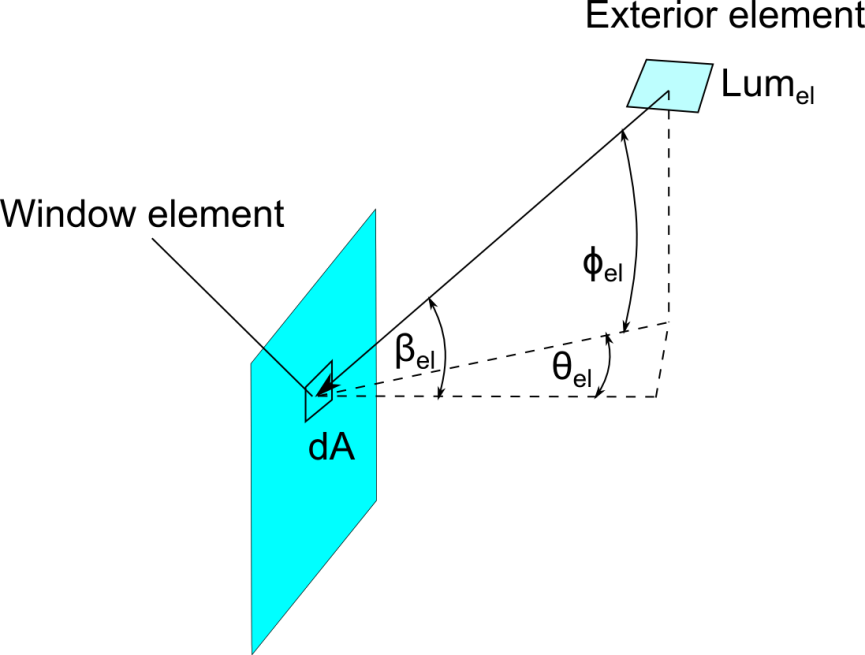
\includegraphics[width=0.9\textwidth, height=0.9\textheight, keepaspectratio=true]{media/image834.png}
\caption{Exterior Luminance Element \protect \label{fig:exterior-luminance-element}}
\end{figure}

This will produce luminous flux at the interior side of the window:

\begin{equation}
d\phi {W_{inside}} = dE{W_{at\_window}} \cdot \tau ({\beta_{el}}) \cdot dA
\end{equation}

where \(dE{W_{at\_window}}\)~is given by Equation~\ref{eq:IlluminanceAtWindowElement}, \(\tau ({\beta_{el}})\)~is the window transmittance at the incoming angle \({\beta_{el}}\)~and \(dA\)~is infinitesimal window element surface area.

Integrating luminous flux given by Equation~\ref{eq:IlluminanceAtWindowElement} over entire window area will give luminous flux on the interior side of the window.

To calculate the interan average reflected illumiance from the window, a simillar approch will be used as described in the chapter ``Internally-Reflected Component of Interior Daylight Illuminance'', which gives the flux balance equation:

\begin{equation}
A \cdot {E_r} \cdot (1 - \rho ) = {F_1}
\end{equation}

where \({F_1}\) represents first reflected flux which in the case of non-CFS is calculated by using the split-flux method.~ In the case of CFS, first the reflected flux can be calculated more precisely by using light patches area.~ Since each CFS is described by a BSDF, it is possible to calculate the light patches for each outgoing direction (see Figure~\ref{fig:complex-fenestration-system-light-patches}).

\begin{figure}[hbtp] % fig 64
\centering

\includegraphics[width=0.9\textwidth, height=0.9\textheight, keepaspectratio=true]{media/image842.png}
\caption{Complex Fenestration System Light Patches \protect \label{fig:complex-fenestration-system-light-patches}}
\end{figure}

Considering the total flux passing through the window at the outgoing direction ``k'', the first reflect flux (\({F_{1,k}}\)) can be calculated as:

\begin{equation}
{F_{1,k}} = {\phi_k} \cdot \frac{{\sum\limits_{a = 1}^N {({A_{overlap,k,a}} \cdot {\rho_{vis,k,a}})} }}{{\sum\limits_{a = 1}^N {{A_{overlap,k,a}}} }}
\end{equation}

where \({\phi_k}\) ~is the total flux entering the zone at the BSDF outgoing direction ``k'' and is calculated by integrating Equation~\ref{eq:IlluminanceAtWindowElement} over the entire window area for a given outgoing direction ``k'', N is the number of interior surfaces hit by the BSDF outgoing direction ``k'' (see Figure~\ref{fig:complex-fenestration-system-light-patches}), \({A_{overlap,k,a}}\) ~is the surface (patch) area which the window from the BSDF outgoing direction ``k'' makes at surface ``a'' and \({\rho_{vis,k,a}}\) ~is the visible reflectance from surface ``a''.

Summing all the outgoing directions will result in total first reflected flux:

\begin{equation}
{F_1} = \sum\limits_{k = 1}^{{N_{out}}} {{F_{1,k}}}
\end{equation}

\subsection{Luminance from Exterior Elements}\label{luminance-from-exterior-elements}

The case of CFS luminance from exterior elements can be calculated by using BSDF incoming directions defined for a given CFS.~ Applying Equation~\ref{eq:IlluminanceAtWindowElement} for a certain incoming BSDF direction will give:

\begin{equation}
\Delta E{W_{el,i}} = Lum({\theta_i},{\psi_i}) \cdot \cos ({\beta_i}) \cdot \cos ({\phi_i}) \cdot \Delta {\theta_i} \cdot \Delta {\psi_i}
\end{equation}

This equation can be translated in the BSDF coordinate system where, instead of standard azimuth and altitude angles, the equation will be transformed into the BSDF coordinate system.~ In that case, Equation~\ref{eq:IlluminanceAtWindowElement} becomes:

\begin{equation}
\Delta E{W_{el,i}} = Lum({\theta_i},{\psi_i}) \cdot {\Lambda_i}
\end{equation}

where \({\Lambda_i}\) represents the lambda value for the incoming direction ``i''.

\subsection{Luminous Flux and Direct Illuminance at Interior Side of the Window}\label{luminous-flux-and-direct-illuminance-at-interior-side-of-the-window}

In the case of CFS it is of interest to calculate fluxes for each outgoing BSDF direction.~ For a given amount of illuminance at an incoming direction ``i'', flux into direction ``o'' will be calculated as:

\begin{equation}
\Delta \phi {W_{i,o}} = \Delta E{W_{el}} \cdot {T_{dir - dir,i,o}}
\end{equation}

where \({T_{dir - dir,i,o}}\) ~is the direct-direct transmittance for given incoming and outgoing directions (``i'' and ``o'').

\begin{figure}[hbtp] % fig 65
\centering
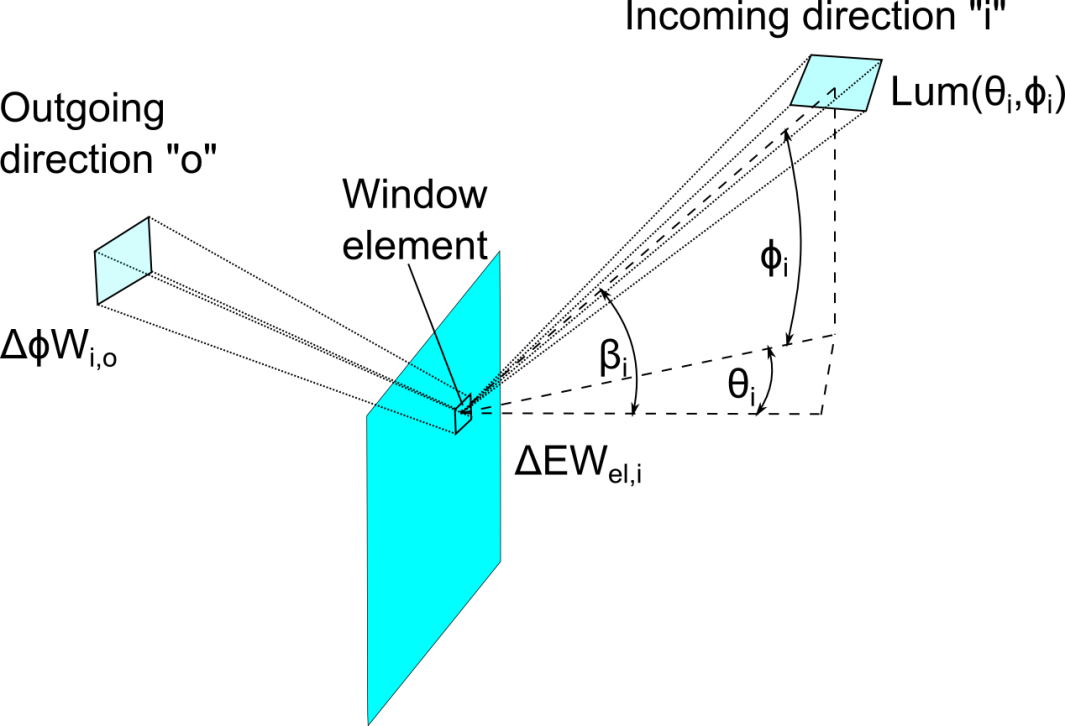
\includegraphics[width=0.9\textwidth, height=0.9\textheight, keepaspectratio=true]{media/image854.png}
\caption{Complex Fenestration System Flux Transition - Single Incoming Direction to Single Outgoing Direction \protect \label{fig:complex-fenestration-system-flux-transition}}
\end{figure}

Total flux from the window at the outgoing direction ``o'' can be calculated by summing over all the incoming directions:

\begin{equation}
\Delta \phi {W_o} = \sum\limits_{i = 1}^{{N_{inc}}} {(\Delta E{W_{el,i}} \cdot {T_{dir - dir,i,o}})}
\end{equation}

where \({N_{inc}}\) ~is the number of BSDF incident directions.

Flux transmitted in the outgoing direction ``o'', calculated by equation , can be used for any given distribution of an exterior luminous element.~ Knowing the intensity of the luminous flux, the direct illuminance at a certain point is calculated as:

\begin{equation}
E{D_o} = \Delta {\Omega_{el}} \cdot \sin ({\phi_{el}}) \cdot \Delta \phi {W_o}
\end{equation}

where \(E{D_o}\) ~is the direct illuminance at the BSDF outgoing direction ``o'', \(\Delta {\Omega_{el}}\) ~is the spatial angle of the element viewed from a certain reference point and \({\phi_{el}}\) ~is the altitude of the window element viewed from the reference point.

\subsection{Handling Exterior Obstructions}\label{handling-exterior-obstructions}

Exterior obstructions are handled for two different cases.~ The first case is to handle obstructions between the luminous element (sky/ground/sun) and the CFS window element. In that case, the direct illuminance at the window element is modified for the product of all the obstruction transmittances between the luminous and window elements, and Equation~\ref{eq:IlluminanceAtWindowElement} is modified as:

\begin{equation}
\Delta E{W_{el,i}} = Lum({\theta_i},{\psi_i}) \cdot {\Lambda_i} \cdot \prod\limits_{p = 1}^{{N_o}} {{\tau_{obs,p}}}
\end{equation}

where \({N_o}\)~is the number of exterior obstructions and \({\tau_{obs,p}}\)~is the visible transmittance of obstruction ``p''.

The second case is to handle all obstructions between the luminous elements and the ground element.~ The luminance from the ground element is calculated as:

\begin{equation}
Lu{m_{gnd}} = \frac{{{E_h}}}{\pi } \cdot {\rho_{gnd}}
\end{equation}

where \({E_h}\)~is the horizontal illuminance and \({\rho_{gnd}}\)~is the ground reflectance.~ Horizontal illuminance is obtained by the integration over sky/sun elements and it is of interest to examine if all elements are visible from a certain ground point.~ The integration examines if the ray between the sky and the ground element is hitting an obstruction.~ It does not take into account whether or not the obstruction is transparent, it simply counts the number of hits.~ The sky obstruction multiplier is calculated as:

\begin{equation}
SOM = \frac{{NumberOfUnobstructedRays}}{{NumberOfRays}}
\end{equation}

and in case the incoming element is from the ground, the illuminance at the window element (Equation~\ref{eq:IlluminanceAtWindowElement}) will be additionally modified from the sky obstruction multiplier:

\begin{equation}
\Delta E{W_{el,i}} = Lum({\theta_i},{\psi_i}) \cdot {\Lambda_i} \cdot SOM \cdot \prod\limits_{p = 1}^{{N_o}} {{\tau_{obs,p}}}
\end{equation}
